\documentclass[conference]{IEEEtran}
%\usepackage{llncsdoc}
\usepackage{graphicx}
\usepackage{amssymb}
\usepackage{algorithm}
\usepackage[noend]{distribalgo}
\usepackage{fixme}
\usepackage{xspace}

\newcommand{\ex}{$\mathcal{E}$}
\newcommand{\pp}{$\mathcal{P}$}
\newcommand{\ppm}{\mathcal{P}}
\newcommand{\cc}{$\mathcal{C}$}
\newcommand{\ccm}{\mathcal{C}}
\newcommand{\vv}{$\mathcal{V}$}
\newcommand{\vvm}{\mathcal{V}}
\newcommand{\vvt}{$\mathcal{V}$}
\newcommand{\rr}{$\mathcal{R}$}
\newcommand{\rrm}{\mathcal{R}}
\newcommand{\sst}{$\mathcal{S}$}
\newcommand{\ssm}{\mathcal{S}}
%
% S-SMR
\newcommand{\ssmr}{\mbox{S-SMR}\xspace}
\newcommand{\ssmrshort}{Scalable SMR}
\newcommand{\ssmrlong}{Scalable State Machine Replication}
%
% DS-SRM
\newcommand{\dssmr}{\mbox{DS-SMR}}
\newcommand{\dssmrshort}{Dynamic S-SMR}
\newcommand{\dssmrlong}{Dynamic Scalable State Machine Replication}
%
% Eyrie and Chirper temporary name (double blind)
\newcommand{\libname}{Nest}    % rename to Eyrie   after paper is accepted
\newcommand{\appname}{Flitter} % rename to Chirper after paper is accepted
%
\newcommand{\rmcast}{reliable-multicast}
\newcommand{\rmdel}{reliable-deliver}
\newcommand{\amcast}{atomic-multicast}
\newcommand{\amdel}{atomic-deliver}
\begin{document}

\title{\dssmrlong}

%\author{[Regular Paper]\\\vspace{20pt}}

\author{
\IEEEauthorblockN{Resarch Paper}
\IEEEauthorblockA{Name of Authors\\Omitted}
}

\author{\IEEEauthorblockN{Long Hoang Le}
\IEEEauthorblockA{University of Lugano\\Switzerland}
\and
\IEEEauthorblockN{Carlos Eduardo Bezerra}
\IEEEauthorblockA{University of Lugano\\Switzerland}
\and
\IEEEauthorblockN{Fernando Pedone}
\IEEEauthorblockA{University of Lugano\\Switzerland}}

\maketitle
\thispagestyle{plain}
\pagestyle{plain}
%

Sharding and replication are the mechanisms of choice of most scalable and fault-tolerant distributed systems.
The performance of a sharded system, however, heavily depends on the partitioning of the data: in order to scale, most commands must involve a single shard and load must be balanced across shards.
Estimating a good partitioning of the application state is challenging since it requires a priori information about the workload.
Moreover, even if such information is available, access patterns may change during system execution.
A good partitioning of the data for uniform access patterns may lead to poor performance under skewed access patterns.
The paper introduces DynaStar, a scalable and fault-tolerant system that supports dynamic state partitioning.
This means that DynaStar does not require a priori knowledge about the workload and can seamlessly adapt to workload variations.
The paper describes DynaStar design and implementation, and presents a detailed performance evaluation using two benchmarks, a social network based on real data and TPC-C.


%!TEX root =  ssmr_ieee.tex

\section{Introduction}
\label{sec:introduction}

Many current online services have stringent availability and performance requirements.
High availability entails tolerating component failures and is typically accomplished with replication.
For many online services, ``high performance" essentially means the ability to serve an arbitrarily large load, something that can be achieved if the service can scale throughput with the number of replicas.
% as the load increases (i.e., as more client requests are submitted by unit of time).
%
State machine replication (SMR)~\cite{Lam78, Sch90} is a well-known technique to provide fault tolerance without sacrificing strong consistency (i.e., linearizability).
%
%\ul{SMR consists of having replicas executing all clients requests in the same order. It usually requires each request execution to be deterministic, in which case the execution will lead to the same state in every replica.} 
SMR regulates how client commands are propagated to and executed by the replicas: every \mbox{non-faulty} replica must receive and execute every command in the same order. Moreover, command execution must be deterministic.
%
SMR provides configurable availability, by setting the number of replicas, but limited scalability: every replica added to the system must execute all requests; hence, throughput does not increase as replicas join the system.

Distributed systems usually rely on state partitioning to scale (e.g., \cite{facebookTAO, sciascia2012sdur}).
If requests can be served simultaneously by multiple partitions, then augmenting the number of partitions results in an overall increase in system throughput.
%, i.e., the system can scale throughput with the number of partitions.
However, exploiting state partitioning in SMR is challenging:
First, ensuring linearizability efficiently when state is partitioned is tricky.  
To see why, note that the system must be able to order multiple streams of commands simultaneously (e.g., one stream per partition) since totally ordering all commands cannot scale.
But with independent streams of ordered commands, how to handle commands that address multiple partitions?
%
Second, SMR hides from the service designer much of the complexity involved in replication; all the service designer must provide is a sequential implementation of each service command.
If state is partitioned, then some commands may need data from multiple partitions.
Should the service designer introduce additional logic in the implementation to handle such cases?
Should the service be limited to commands that access a single partition?

This paper presents Scalable State Machine Replication (S-SMR), an approach that achieves scalable throughput and strong consistency (i.e., linearizability) without constraining service commands or adding additional complexity to their implementation.
%
S-SMR partitions the service state and relies on an atomic multicast primitive to consistently order commands within and across partitions.
We show in the paper that simply ordering commands consistently across partitions is not enough to ensure strong consistency in partitioned state machine replication.
S-SMR implements \emph{execution atomicity}, a property that prevents command interleaves that violate strong consistency. 
%Together with atomic multicast, it ensures linearizability for S-SMR (a detailed description is given in Section~\ref{sec:scalablesmr}).
%
To assess the performance of S-SMR, we developed Eyrie, a Java library that allows developers to implement partitioned-state services transparently, abstracting partitioning details, and Volery, a service that implements Zookeeper's API~\cite{ZOO2010}. 
All communication between partitions is handled internally by Eyrie, including remote object transfers. 
%To evaluate both S-SMR and the library, we used Eyrie to implemented Volery, a service that provides some functionalities of Zookeeper~\cite{ZOO2010}. 
In the experiments we conducted with Volery, throughput scaled with the number of partitions, in some cases linearly.
%, reaching 8 times the throughput of a single-partition Volery deployment when using 8 partitions. 
In some deployments, Volery reached over 250 thousand commands per second, largely outperforming Zookeeper, which served 45 thousand commands per second under the same workload.


The paper makes the following contributions: 
(1)~It introduces S-SMR and discusses several performance optimizations, including caching techniques.
(2)~It details Eyrie, a library to simplify the design of services based on S-SMR. 
(3)~It describes Volery to demonstrate how Eyrie can be used to implement a service that provides Zookeeper's API.
(4)~It presents a detailed experimental evaluation of Volery and compares its performance to Zookeeper.

The remainder of this paper is organized as follows.
Section~\ref{sec:model} describes our system model.
Section~\ref{sec:smr} presents state-machine replication and the motivation for this work.
Section~\ref{sec:scalablesmr} introduces S-SMR; we explain the technique in detail and argue about its correctness.
Section~\ref{sec:implementation} details the implementation of Eyrie and Volery.
Section~\ref{sec:evaluation} reports on the performance of the Volery service.
Section~\ref{sec:related_work} surveys related work and
Section~\ref{sec:conclusion} concludes the paper.

\clearpage
\section{System model and definitions}
\label{sec:sysmodel}

We consider a distributed system consisting of an unbounded set of client processes $\ccm = \{c_1, c_2, ...\}$ and a bounded set of server processes (replicas) $\ssm = \{s_1, ..., s_n\}$. 
Set $\ssm$ is divided into disjoint groups of servers $\ssm_0, ..., \ssm_k$.
Processes are either \emph{correct}, if they never fail, or \emph{faulty}, otherwise. 
In either case, processes do not experience arbitrary behavior (i.e., no Byzantine failures).

Processes communicate by message passing, using either one-to-one or one-to-many communication.
The system is asynchronous: there is no bound on message delay or on relative process speed.
One-to-one communication uses primitives $send(p,m)$ and $receive(m)$, where $m$ is a message and $p$ is the process $m$ is addressed to. 
If sender and receiver are correct, then every message sent is eventually received. 
%
One-to-many communication relies on reliable multicast and atomic multicast,\footnote{Solving atomic multicast requires additional assumptions~\cite{CT96,FLP85}. In the following, we simply assume the existence of an atomic multicast oracle.}
defined in sections~\ref{sec:rmcast} and \ref{sec:amcast}, respectively.
%Atomic broadcast is a special case of atomic multicast in which there is a single group with all servers.

Our consistency criterion is linearizability.
A system is \emph{linearizable} if there is a way to reorder the client commands in a sequence that (i)~respects the semantics of the commands, as defined in their sequential specifications, and (ii)~respects the real-time precedence of commands~\cite{Attiya04}.

\subsection{Reliable multicast}
\label{sec:rmcast}

To reliably multicast a message $m$ to a set of groups $\gamma$, processes use primitive \rmcast$(\gamma, m)$.
Message $m$ is delivered at the destinations with \rmdel$(m)$.
Reliable multicast has the following properties:

\begin{itemize}

    \item[--] If a correct process \rmcast{}s $m$, then every correct process in $\gamma$ \rmdel{}s $m$ \emph{(validity)}.
    
    \item[--] If a correct process \rmdel{}s $m$, then every correct process in $\gamma$ \rmdel{}s $m$ \emph{(agreement)}.
    
    \item[--] For any message $m$, every process $p$ in $\gamma$ \rmdel{}s $m$ at most once, and only if some process has \rmcast{} $m$  to $\gamma$ previously \emph{(integrity)}.
    
\end{itemize}

\subsection{Atomic multicast}
\label{sec:amcast}

To atomically multicast a message $m$ to a set of groups $\gamma$, processes use primitive \amcast$(\gamma, m)$.
Message $m$ is delivered at the destinations with \amdel$(m)$.
Atomic multicast ensures the following properties:

\begin{itemize}
    
    \item[--] If a correct process \amcast{}s $m$, then every correct process in $\gamma$ \amdel{}s $m$ \emph{(validity)}.
    
    \item[--] If a process \amdel{}s $m$, then every correct process in $\gamma$ \amdel{}s $m$ \emph{(uniform agreement)}.
    
    \item[--] For any message $m$, every process $p$ in $\gamma$ \amdel{}s $m$ at most once, and only if some process has \amcast{} $m$ to $\gamma$ previously \emph{(integrity)}.
    
    \item[--] No two processes $p$ and $q$ in both $\gamma$ and $\gamma'$ \amdel\ $m$ and $m'$ in different orders; also, the delivery order is acyclic \emph{(atomic order)}.
    
\end{itemize}

Atomic broadcast is a special case of atomic multicast in which there is a single group of processes.
\section{Background and motivation}
State-machine replication is a fundamental approach to implement a fault-tolerant service by replicating servers and coordinating the execution of client commands against server replicas~\cite{Lam78,Sch90}. 
State-machine replication ensures strong consistency (i.e., linearizability~\cite{Attiya04}) by coordinating the execution of commands in the different replicas: Every replica has a full copy of the service state $\vvm = \{v_1, ..., v_m\}$ and executes commands submitted by the clients in the same order. A command is a program consisting of a sequence of operations, which can be of three types: \emph{read(v)}, \emph{write(v, val)}, or a deterministic computation.

\subsection{Scaling state-machine replication}
By starting in the same initial state and executing the same sequence of deterministic commands, servers make the same state changes and produce the same reply for each command. To guarantee that servers deliver the same sequence of commands, SMR can be implemented with atomic broadcast: commands are atomically broadcast to all servers, and all correct servers deliver and execute the same sequence of commands \cite{BJ87b,DSU04}.

Despite its simple execution model, classical SMR does not scale: adding resources (e.g., replicas) will not translate into sustainable improvements in throughput. This happens for a few reasons. First, the underlying communication protocol needed to ensure ordered message delivery may not scale itself (i.e., a communication bottleneck). Second, every command must be executed sequentially by each replica (i.e., an execution bottleneck).

Several approaches have been proposed to address SMR’s scalability limitations. To cope with communication overhead, some proposals have suggested to spread the load of ordering commands among multiple processes (e.g., \cite{Moraru:2013gw,Mencius,Marandi:2012hb}), as opposed to dedicating a single process to determine the order of commands (e.g., \cite{CT96,Lamport:1998ea}).

Two directions of research have been suggested to overcome execution bottlenecks. One approach (scaling up) is to take advantage of multiple cores to execute commands concurrently without sacrificing consistency \cite{Kapritsos:2012um,Marandi:2014bj,Kotla:2004ep,Guo:2014jp}. Another approach (scaling out) is to partition the service's state and replicate each partition (e.g., \cite{Glendenning:2011kj,Marandi:2011dj}. In the following section, we review Scalable State-Machine Replication (S-SMR), a proposal in the second category.

\subsection{Scalable State-Machine Replication}
TODO: talk about SSMR

SSMR implementation brings into use the concept of \emph{Oracle}, the core of partitioning algorithms, which runs a static deterministic algorithm to return the combination of involved partitions of a command; all clients and partitions have their own version of Oracle, and assumed to be identical. By doing that way, SSMR can ensure Oracle return same results for query from both clients and partitions. However, this implementation leads to some limitations: (i) the Oracles on all parties are not synchronized, thus they need to have the knowledge of all $v \in \vvm$ during the life-cycle of the system, and (ii) a change in $\vvm$ on one Oracle will not be recognized by the others. Therefore, SSMR doesn't support creating state variable $v_n$ on the fly, and has to initialize the whole $\vvm$ on the starting phase.

\section{Dynamic Scalable State Machine Replication}

In this section, we introduce Dynamic SSMR, discuss performance optimizations, and argue about D-SSMR's correctness.

\subsection{General idea}
\label{sec:generalidea}

S-SMR divides the state variables $v$ into $P$ partitions $\ppm_1, ..., \ppm_P$, where for each $\ppm_i$, $\ppm_i \subseteq \vvm$, and each variable $v$ in $\vvm$ has to be assigned to at least one partition and define $part(v)$ as the partitions that hold $v$. Each partition $\ppm_i$ is replicated by servers in group $s_i$. For brevity, the server $s$ belongs to $\ppm_i$ with the meaning that $s \in \ssm_i$, and say that client $c$ multicasts command $C$ to partition $\ppm_i$ means that $c$ multicasts $C$ to group $\ssm_i$.

To execute command $C$, the client multicasts $C$ to all partitions that hold a variable read or updated by $C$.
Consequently, the client must be able to determine the partitions accessed by $C$, denoted by $part(C)$. If the client cannot accurately estimate which partitions are accessed by $C$, it must determine a superset of these partitions, in the worst case assuming all partitions.
In order for clients to provide a close approximation to the command's actually accessed partitions, there is an oracle that tells the client which partitions should receive each command.

Dynamic SSMR improves on SSMR implementation by adding a central Oracle which has the information of all state variables $\vvm$, as well as provides a mechanism of controlling the access to those variable that ensure linearizability. 

We distinguish between three operation types: $read(v)$, an operation that reads the value of a state variable, $v$, $create(v, P)$, an operation that create a state variable at a specific partition P, and $move(v, \ppm_n)$, an operation that move $v$ to partition $\ppm_n$.

Consider the execution depicted in Figure~\ref{fig:read}~(a), where state variables $x$ is created on partition $\ppm_1$ in the middle of the execution of SSMR. Command $C_1(x)$ and $C_3(x)$ reads the value of $x$, $C_2(x,\ppm_1)$ create $x$ on partition $\ppm_1$. Client a first multicasts query to the $Oracle$ for location of $x$, which is not available at that time, hence $Oracle$ return empty result, which tell client a to end the execution. Client b then wants to create variable $x$ on $\ppm_1$, before sending actual creating command, client b also multicasts query to $Oracle$ to get the involved partition (eg., $\ppm_1$), then multicasts $C_2(x,\ppm_1)$ to both $Oracle$ and $\ppm_1$. Oracle will update information of $x$, and $\ppm_1$ will execute create $x$ command. From then, for every read command to $x$ (eg., $C_3(x)$), $Oracle$ could answer with partition $\ppm_1$ which is the one holds $x$.

\begin{figure*}
\begin{minipage}[b]{1.0\linewidth} % A minipage that covers the whole width of the page
\centering
      \includegraphics[width=0.6\linewidth]{figures/read_simple}
\end{minipage}
\centering
	\caption{Execution flow of D-SSMR with $create$ command}
\label{fig:read}
\end{figure*}

In the following figures~(\ref{fig:readoverlap}b, \ref{fig:readoverlap}c), where read command $C_1(x)$ comes in the middle of the execution of create command $C_2(x,\ppm_1)$, while the query of $C_1(x)$ comes after multicasts command of $C_2(x,\ppm_1)$. With the knowledge of $x$, Oracle response to the query with a positive answer, therefore there are possibilities that the read command either comes during (eg., fig.~\ref{fig:readoverlap}b) or before (eg., fig.~\ref{fig:readoverlap}c) the execution of actual write command. The SSMR model avoid the problem described in figure~\ref{fig:readoverlap}~(b) by ensuring that the execution of every command is atomic (eg., for every server $s$ in partition $\ppm$ that executes $C$, there is a server $r$ in every $\ppm' \in part(C)$ such that $delivery(C,r) < end(C,s)$. Intuitively, this condition guarantees that the execution of $C_1$ and $C_2$ at $\ppm$ overlap in time). Atomic multicast prevents the problem figure~\ref{fig:readoverlap}~(c) from happening as $deliver(C_2) \prec deliver(C_1)$, that leads to situation described in fig.~\ref{fig:readoverlap}b.

\begin{figure*}
\begin{minipage}[b]{1.0\linewidth} % A minipage that covers the whole width of the page
\centering
      \includegraphics[width=1\linewidth]{figures/read_overlap}
\end{minipage}
\caption{Execution flow of D-SSMR with overlapping read-create commands}
\label{fig:readoverlap}
\end{figure*}


Next figure~(\ref{fig:updateoverlap} a, \ref{fig:updateoverlap} b) depicts the scenario of moving object location from a partition to another. Intuitively, the problem with the execution in fig.~\ref{fig:updateoverlap}a is that read command $C_3(x)$ executes “in between” the execution of $C_2(x,\ppm_2)$ at partitions Px and Py. Before sending $C_3$ to destination partition, client 1 send query to oracle for possible position of $x$, which is $P_1$ at that specific moment, but not correct at the execution time. In D-SSMR, we prevent that from happening by using oracle as the controller for accessing state variable on partitions, by using locking mechanism on oracle for different type of commands. Whenever a client sends a query variable's location $Q(x)$ from oracle for a command $C$, it also requires a lock $L(x)$. Then after the associated process execute command $C$, it also tell Oracle to release the lock $L$, and inform the oracle about the update of $x$ (if there is any).

There are possibilities that a client could fail in the middle of the execution of the command chains, at the moment after requires the lock and before sending the actual $C$ command to partition $P$. In this case, TODO: which one release lock, either oracle or another client that require lock again. 

\begin{figure*}
\begin{minipage}[b]{1.0\linewidth} % A minipage that covers the whole width of the page
\centering
      \includegraphics[width=1\linewidth]{figures/update_overlap}
\end{minipage}
\caption{Execution flow of D-SSMR with overlapping read-update commands}
\label{fig:updateoverlap}
\end{figure*}


\subsection{Detailed algorithm}
\label{sec:detailalg}

In Algorithm \ref{alg:dssmr}, we show the basic operation of D-SSMR. 
To submit a command $C$, the client queries an oracle to get set $dests$~(line \ref{algline:query_oracle}, \ref{algline:oracle_response}), which is a superset of $part(C)$ used by the client as destination set for $C$~(line \ref{algline:cli_mcast}). If the $dests$ is empty, client stop the command there. (line \ref{algline:cli_terminate})

Upon delivering $Q(C)$, oracle $O$ runs function $getPart(C)$ which returns a set $\vvm$ of involved state variables of command $C$. If there exists a variable $v_i \in \vvm$ in oracle memory, which indicates the variable $v_i$ exists on a partition $p_i \in \ppm$, oracle reply to client with $p_i$ value, or an empty result otherwise. In addition, upon delivering $C(v, \ppm)$, oracle update its memory with new location of $v$: $\vvm\_loc\{v.id\} \leftarrow \ppm$

Upon delivering $C$, server $P$ execute $C$ and reply to the client. 
% Upon delivering $C$, server $s$ in partition \pp\ multicasts $signal(C)$ to $others$, which is the set containing all other partitions involved in $C$ (lines \ref{algline:others} and \ref{algline:mcastsignals}). 
% %The purpose of $signal(C)$ is to let servers in other partitions know that there is a server in \pp\ that started executing $C$. 
% It might happen that $s$ receives signals concerning $C$ from other partitions even before $s$ started executing $C$. For this reason, $s$ must buffer signals and check if there are signals buffered already when starting the execution of $C$. For the sake of simplicity, Algorithm \ref{alg:ssmr} simply initializes such buffers as $\emptyset$ for all possible commands. In practice, buffers for $C$ are created when the first message concerning $C$ is delivered.

% After multicasting signals, server $s$ proceeds to the execution of $C$, which is a sequence of operations that might read or write variables in \vv. The main concern is with operations that read variables, as they may determine the outcome of the command execution. All other operations can be executed locally at $s$. If the operation reads variable $v$ and $v$ belongs to \pp, $s$'s partition, then $s$ multicasts the value of $v$ to the other partitions that delivered $C$ (line \ref{algline:multicastv}). The command identifier $C.id$ is sent along with $v$ to make sure that the other partitions will use the appropriate value of $v$ during $C$'s execution. If $v$ belongs to some other partition $\ppm'$, $s$ waits until an up-to-date value of $v$ has been delivered (line \ref{algline:waitvariable}). Every other operation is executed with no interaction with other partitions (line \ref{algline:executeopck}).

% After executing all operations of $C$, $s$ waits until a signal from every other partition has been received (line \ref{algline:waitsignals}) and, only then, sends the reply back to the client (line \ref{algline:sendreply}). This ensures that $C$ will be execution atomic.



% Upon delivering $C$, server $s$ in partition \pp\ multicasts $signal(C)$ to $others$, which is the set containing all other partitions involved in $C$ (lines \ref{algline:others} and \ref{algline:mcastsignals}). 
% %The purpose of $signal(C)$ is to let servers in other partitions know that there is a server in \pp\ that started executing $C$. 
% It might happen that $s$ receives signals concerning $C$ from other partitions even before $s$ started executing $C$. For this reason, $s$ must buffer signals and check if there are signals buffered already when starting the execution of $C$. For the sake of simplicity, Algorithm \ref{alg:dssmr} simply initializes such buffers as $\emptyset$ for all possible commands. In practice, buffers for $C$ are created when the first message concerning $C$ is delivered.


\begin{algorithm}
\small
%\footnotesize
\begin{distribalgo}[1]
%\STATE \textbf{Algorithm 1:\\} Scalable State-Machine Replication (S-SMR)
\vspace{1mm}

\INDENT{\emph{Initialization:}}
    \STATE  oracle: $\vvm\_loc \leftarrow \emptyset$
    % \STATE $\forall C \in \mathcal{K} : rcvd\_signals(C) \leftarrow \emptyset$
    % \STATE $\forall C \in \mathcal{K} : rcvd\_variables(C) \leftarrow \emptyset$
\ENDINDENT

\vspace{1.5mm}

\INDENT{\emph{Command $C$ is submitted by a client as follows:}}
	\STATE multicast query $Q(oracle, C)$ \label{algline:query_oracle} 
    \STATE $dests \leftarrow O(C)$ \label{algline:oracle_response} 
    \IF {$dests$ is $\emptyset$}
    	\STATE terminate $C$ \label{algline:cli_terminate}
    \ELSE
    	\STATE multicast$(dests, C)$ \label{algline:cli_mcast}
    	\STATE wait for response from one server
    \ENDIF
%    \COMMENT{$oracle(C)$ returns a superset of $part(C)$}
\ENDINDENT

\vspace{1.5mm}

\INDENT{\emph{Command $C$ is executed by a oracle as follows:}}
	\INDENT{\textbf{upon} deliver $Q(C)$}
		\STATE $v \leftarrow get part(C)$
		\IF {$v$ in $\vvm\_loc$}
			\STATE send reply to client $\vvm\_loc\{v.id\}$
		\ELSE
			\STATE send reply to client $\emptyset$
		\ENDIF
	\ENDINDENT

	\INDENT{\textbf{upon} deliver $C(v, \ppm)$}
		\STATE $\vvm\_loc\{v.id\} \leftarrow \ppm$
	\ENDINDENT

\ENDINDENT

\vspace{1.5mm}
\emph{TODO: Should give the detail algorithm of SSMR? or give short description of dssmr}
\vspace{1.5mm}

\INDENT{\emph{Command $C$ is executed by a server in partition \pp\ as follows:}}
	\INDENT{\textbf{upon} deliver$(C)$}	    
		\STATE execute $op$ \label{algline:executeopck}
		\STATE send reply to client \label{algline:sendreply}
	\ENDINDENT
\ENDINDENT

% \INDENT{\emph{Command $C$ is executed by a server in partition \pp\ as follows:}}
% 	\INDENT{\textbf{upon} deliver$(C)$}
% 	    \STATE $others \leftarrow dests \setminus \{\ppm\}$ \label{algline:others}
% 	    \STATE multicast$(others, signal(C))$ \label{algline:mcastsignals}
% 		\FOR{each operation $op$ in $C$}
% 			\IF{$op$ is $read(v)$}
% 			    \IF{$v \in \ppm$}
% 			        \STATE multicast$(others, \{v,C.id\})$ \label{algline:multicastv}
% 			    \ELSE
% 			        \STATE \textbf{wait until} $v \in rcvd\_variables(C)$ \label{algline:waitvariable}
% 			        \STATE update $v$ with the value in $rcvd\_variables(C)$
% 			    \ENDIF
% 			\ENDIF
% 			\STATE execute $op$ \label{algline:executeopck}
% 		\ENDFOR
% 		\STATE \textbf{wait until} $rcvd\_signals(C) = others$ \label{algline:waitsignals}
% 		\STATE send reply to client \label{algline:sendreply}
% 	\ENDINDENT
	
% 	\vspace{2.0mm}
% 	\INDENT{\textbf{upon} deliver$(signal(C))$ from partition $\ppm'$}
% 	    \STATE $rcvd\_signals(C) \leftarrow rcvd\_signals(C) \cup \{\ppm'\}$
% 	\ENDINDENT

% 	\vspace{2.0mm}
% 	\INDENT{\textbf{upon} deliver$(\{v, C.id\})$}
% 	    \STATE $rcvd\_variables(C) \leftarrow rcvd\_variables(C) \cup \{v\}$
% 	\ENDINDENT
			
% \ENDINDENT

\vspace{1.5mm}
%\vspace{2mm}

\textbf{Algorithm variables:}

\vspace{1mm}

$\vvm\_loc$: the set of locations of all state variables in the system.

\vspace{1mm}

$Q(oracle, C)$: multicast command to oracle for querying involved partition of command C

\vspace{1mm}

$O(C)$: response of oracle that returns a superset of $part(C)$

\vspace{1mm}

$dests$: set of partitions to which $C$ is multicast

\vspace{1mm}

$C(v, \ppm)$: command that create variable $v$ in partition $\ppm$

% \vspace{1mm}

% $others$: set of partitions waiting for signals and variables from \pp; also, \pp\ waits for signals from all such partitions

% \vspace{1mm}

% $signal(C)$: a synchronization message that allows S-SMR to ensure $C$ to be execution atomic

% \vspace{1mm}

% $rcvd\_signals(C)$: a set containing all partitions that already signaled \pp\ regarding the execution of $C$

% \vspace{1mm}

% $rcvd\_variables(C)$: a set containing all variables that must be received from other partitions in order to execute $C$

\caption{Dynamic Scalable State-Machine Replication (D-SSMR)}
\label{alg:dssmr}
\end{distribalgo}
\end{algorithm}

\subsection{Performance optimizations}
\label{sec:optm}
TODO: add content, talk about caching

Algorithm 1 can be optimized in many ways. In this section, we briefly mention some of these optimizations and then detail caching.

\begin{figure*}
\begin{minipage}[b]{1\linewidth} % A minipage that covers the whole width of the page
\centering
      \includegraphics[width=0.85\linewidth]{figures/cache}
\end{minipage}
\caption{Execution flow of D-SSMR with oracle caching on client}
\label{fig:cache}
\end{figure*}


\subsection{Correctness}
\label{sec:correctness}
TODO: add content
%!TEX root =  ssmr_ieee.tex
\section{Implementation}
\label{sec:implementation}

In this section, we describe Eyrie, a library that implements S-SMR, and Volery, a service that provides Zookeeper's API.
Volery can be configured to provide high availability by means of state-machine replication and to use Eyrie to combine high availability and throughput scalability.
Volery was built with Eyrie, combining high availability and throughput scalability (by means of scalable state-machine replication).
Both Eyrie and Volery were implemented in Java.
%In this section, we detail the implementation of Eyrie, a library that implements Scalable State-Machine Replication (Section \ref{sec:libjssmr}) and present Volery, an application that provides the Zookeeper API (Section \ref{sec:zkssmr}).
%%Volery can be configured to provide high availability by means of state-machine replication and to use Eyrie to combine high availability and throughput scalability.
%Volery was built with Eyrie, combining high availability and throughput scalability (by means of scalable state-machine replication).
%Both Eyrie and Volery were implemented in Java.

%, Section \ref{sec:zkssmr}) and Chirper (a Twitter-like application, Section \ref{sec:chirper}).
% There are two main aspects of it to consider: (i) how it handles communication between partitions to ensure linearizability and (ii) how transparent it is for developers to migrate an existing fully-replicated service to Scalable SMR.

\subsection{Eyrie}
\label{sec:libjssmr}

One of the main goals of Eyrie is to make the implementation of services based on Scalable SMR as easy as possible. 
To use Eyrie, the user (i.e., service designer) must extend two classes, \verb#PRObject# and \verb#StateMachine#. 
%Even though they are simple to implement, their implementation is required by Eyrie. 
Class \verb#PartitioningOracle# has a default implementation, but the user is encouraged to override its methods. 
%Finally, the user must provide a configuration file describing the partitions and the atomic multicast protocol to be used.



\subsubsection{The \texttt{PRObject} class}

Eyrie supports partial replication (i.e., some objects may be replicated in some partitions, not all). 
Therefore, when executing a command, a replica might not have local access to some of the objects involved in the execution of the command. 
%
%The user informs Eyrie which object classes are partially replicated by extending the \verb#PRObject# class.
The user informs to Eyrie which object classes are partially replicated by extending the \verb#PRObject# class. Each object of such class may be stored locally or remotely, but the application code is agnostic to that. All calls to methods of such objects are intercepted by Eyrie, transparently to the user.

%Eyrie uses AspectJ\footnote{http://eclipse.org/aspectj} to intercept method calls for all subclasses of \verb#PRObject#, which correspond to remote objects. 
%Internally, the aspect related to such remote method invocations communicates with the user's subclass of \verb#StateMachine# in order \fixme{Too vague; what's done really?}to find out what is the command being executed at the moment \ul{and make sure that the execution is linearizable.}

Eyrie uses AspectJ\footnote{http://eclipse.org/aspectj} to intercept method calls for all subclasses of \verb#PRObject#. 
Internally, the aspect related to such method invocations communicates with the \verb#StateMachine# instance in order to (i) determine if the object is stored locally or remotely and (ii) ensure that the object is up-to-date when each command is executed.

Each replica has a local copy of all \verb#PRObject# objects. 
When a remote object is received, replicas in the local partition $P_L$ must update their local copy of the object with an up-to-date value. 
For this purpose, the user must provide implementations for the methods \verb#getDiff(Partition p)# and \verb#updateFromDiff(Object diff)#. The former is used by the remote partition $P_R$, which owns the object, to calculate a delta between the old value currently held by $P_L$ and the newest value, held by $P_R$. Such implementations may be as simple as returning the full object, which is then serialized and, upon deserialization in $P_L$, completely overwrites the old copy of the object. However, it also allows the user to implement caching mechanisms. Since \verb#getDiff# takes a partition as parameter, the user may keep track of what was the last value received by $P_L$, and then return a (possibly small) diff, instead of the whole object, which is then applied to the object with the user-provided method \verb#updateFromDiff#.

%The \verb#PRObject# class also contains several methods that are used internally by Eyrie. For instance, it contains an index of all PRObjects in the system, along with their corresponding partitions. By having such knowledge, each object knows where its up-to-date copy is, so that they can always have recent up-to-date values.

To avoid unnecessary communication, the user may optionally mark some methods of their \verb#PRObject# subclasses as local, by annotating them with \verb#@LocalMethodCall#. Calls to such methods are not intercepted by the library, sparing communication when the user sees fit. Although the command that contains a call to such a method still has to be delivered and executed by all partitions that hold objects accessed by the command, that particular local method does not require an up-to-date object. For example, say a command $C$ accesses objects $O_1$ and $O_2$, respectively, in partitions $P_1$ and $P_2$. $C$ completely overwrites objects $O_1$ and $O_2$, by calling \verb#O1.clear()# and \verb#O2.clear()#. Although $C$ has to be delivered by both partitions to ensure linearizability, a write method that completely overwrites an object, regardless of its previous state, does not need an up-to-date version of the object before executing. Because of this, method \verb#clear()# can be safely annotated as local, avoiding unnecessary communication between $P_1$ and $P_2$.


\subsubsection{The \texttt{StateMachine} class}

This class must be extended by the user's application server class. To execute commands, the user must provide an implementation for the method \verb#executeCommand(Command c)#. The code for such a method is agnostic to the existence of partitions. In other words, it can be exactly the same as the code used to execute commands with classical state-machine replication (i.e., full replication).
Eyrie is responsible for handling all communication between partitions transparently. 
To start the server, method \verb#runStateMachine()# is called.

%Internally,\fixme{This paragraph is too complex.} the \verb#StateMachine# class hands each command multicast by clients to the user's method \verb#executeCommand#. For each executed command, it keeps track of what 
%\verb#PRObject#s have been sent or received already. Each object needs to be updated only once for each command execution, even if it is changed after being received, since all involved replicas perform the same changes on up-to-date objects. Because of this, \verb#StateMachine# makes sure that multiple calls to methods in the same object do not incur multiple object exchanges between partitions.



%Finally, \verb#StateMachine# ensures linearizability by making sure that each command is execution atomic (as defined in Section \ref{sec:generalidea}). 
%A command can only conclude its execution after is has received a signal from at least one server in every other partition that delivered the command---remote object updates received from other partitions count as signals for linearizability purposes.
%
%Both for object updates and signaling among partitions, it is sufficient to have it done by a single replica in each partition. \verb#StateMachine# is implemented this way in order to reduce communication. If a certain replica is responsible for sending a signal or object updates concerning a certain command and such replica fails, other replicas in the same partition will suspect  the failure and one of the operational replicas will retransmit the information.

\verb#StateMachine# ensures linearizability by making sure that each command is execution atomic (as defined in Section \ref{sec:generalidea}). 
As soon as each command $C$ is delivered, \verb#StateMachine# sends $signal(C)$ to all remote partitions that deliver $C$, in order to reduce waiting time.
A command can only conclude its execution after it has received a signal from at least one server in every other partition that delivered the command---remote object updates received from other partitions count as signals for linearizability purposes.
%
%Both for object updates and signaling among partitions, it is sufficient to have it done by a single replica in each partition. \verb#StateMachine# is implemented this way in order to reduce communication. If a certain replica is responsible for sending a signal or object updates concerning a certain command and such replica fails, other replicas in the same partition will suspect  the failure and one of the operational replicas will retransmit the information.
%
%In order to reduce communication, a single replica in each partition sends object updates and signal messages to other partitions.
%If the designated replica fails, the other replicas in the same partition will suspect the failure and one of the operational replicas will retransmit the information.


In order to reduce communication, it is sufficient that a single replica in each partition sends object updates and signal messages to other partitions.
If the designated replica fails, the other replicas in the same partition will suspect the failure and one of the operational replicas will retransmit the information.


\subsubsection{The \texttt{PartitioningOracle} class}

Clients multicast each command directly to the partitions affected by the command, i.e., those that contain objects accessed by the command. 
Although Eyrie encapsulates most details regarding partitioning, the user must provide an oracle that tells, for each command, which partitions are affected by the command. 
The set of partitions returned by the oracle needs to contain all partitions involved, but does not need to be minimal. 
In fact, the default implementation of the oracle simply returns all partitions for every command, which although correct, is not efficient. 
For best performance, the partition set returned by the oracle should be as small as possible, which requires the user to extend \verb#PartitioningOracle# and override its methods.

Method \verb#getDestinations(Command c)# is used by the oracle to tell what partitions should receive each command. It returns a list of \verb#Partition# objects. 
The user can override this method, which will parse command \verb#c# and return a list containing all partitions involved in the execution of \verb#c#. The \verb#getDestinations# method can encapsulate any kind of implementation, including one that involves communicating with servers, so its execution does not necessarily need to be local to clients. If the set of partitions involved in the execution of a command cannot be determined a priori, the oracle can communicate with servers to determine such set and then return it to the client, which then multicasts the command to the right partitions.

Another important method in \texttt{PartitioningOracle} is \verb#getLocalObjects(Command c)#\!, which is used by servers before executing \verb#c#.
The method returns a list of objects in the partition of the server that will be accessed by \verb#c#. 
This list does not need to be complete, but any kind of early knowledge about what objects need to be updated in other partitions helps decrease execution time, as the objects can be sent as soon as the server starts executing the command. The default implementation of this method returns an empty list, which means that objects are exchanged among partitions as their methods are invoked during execution. Depending on the application, the user may provide an implementation for this method.


\subsubsection{Other classes}
In the following, we briefly describe a few accessory classes provided by Eyrie.

The \verb#Partition# class %is an abstraction provided by Eyrie. 
%Even though it is of fundamental importance for Eyrie internally, all the user has to care about are its 
has two relevant methods, \verb#getId()# and \verb#getPartitionList()#, which return, respectively, the partition's unique identifier and the list of all partitions in the system.
The oracle can use this information to map commands to partitions.

When sending commands, the client must multicast a \verb#Command# object, which is serialized and sent to the partitions determined by the client's oracle. To the user, a command object is simply a container of objects, which are typically parameters for the command. The \verb#Command# class offers methods \verb#addItems(Objects... objs)#, \verb#getNext()#, \verb#hasNext()# and so on. How the server will process such parameters is application-dependent and determined by %the \verb#executeCommand# method of
the user's implementation of \verb#StateMachine#.

Eyrie uses atomic multicast to disseminate commands from clients and handle communication between partitions.
%This is done by configuring a \verb#LocalReplica# object, which is created by parsing a configuration file provided by the user, in both clients and servers.
Internally, it uses an implementation\footnote{https://github.com/sambenz/URingPaxos} of Multi-Ring Paxos~\cite{MRPPROC2012}. To map rings to partitions, each server in partition $\ppm_i$ is a learner in rings $\rrm_i$ and $\rrm_{all}$ (merge is deterministic); if message $m$ is addressed only to $\ppm_i$, $m$ is sent to $\rrm_i$, otherwise, to $\rrm_{all}$ (and discarded by non-addressee partitions). 

%Internally, the \verb#LocalReplica# object instantiates a \verb#MulticastAgent#, which is an interface that provides an atomic multicast API. It is provided by \mbox{Libmcad},
%%\footnote{https://bitbucket.org/kdubezerra/libmcad}
%a multicast adaptor library bundled together with Eyrie. By default, \verb#LocalReplica# uses an implementation of \verb#MulticastAgent# provided by Libmcad that internally uses URingPaxos,\footnote{https://github.com/sambenz/URingPaxos} a Java implementation of Multi-Ring Paxos . We configured the atomic multicast algorithm with batching enabled: each client sends its commands to a ring coordinator, which will batch commands, possibly from multiple clients, and order the batch when it reaches a certain batch size or a timer expires.
%wait for (i) a timeout or (ii) a certain batch size threshold to be reached, whatever comes first. 
%Even though this obviously introduces latency, it allows the system throughput to increase more than it would without batching.


%The user is also free to provide a custom multicast agent, by implementing methods \verb#multicast(groups, message)# and \verb#deliver()#, and passing the custom agent to the \verb#LocalReplica# object.

\subsection{Volery}
\label{sec:zkssmr}

We implemented the Volery service on top of Eyrie, providing an API similar to that of Zookeeper~\cite{ZOO2010}. 
%Zookeeper has been designed to provide high throughput and high availability, among other properties that make it interesting to be used by other system as a central coordinator. It is used by many systems, including several Apache projects and Yahoo! services.\footnote{https://cwiki.apache.org/confluence/display/ZOOKEEPER/PoweredBy}
%
ZooKeeper implements a hierarchical key-value store, where each value is stored in a znode, and each znode can have other znodes as children. 
The abstraction implemented by ZooKeeper resembles a file system, where each path is a unique string (i.e., a key) that identifies a znode in the hierarchy. 
We implemented the following Volery client API:
%The Volery client API we implemented was the following:

\begin{itemize}

\item \verb#create(String path, byte[] data)#: creates a znode with the given \verb#path#, holding \verb#data# as content, if there was no znode with that path previously and there is a znode with the parent path.

\item \verb#delete(String path)#: deletes the znode that has the given \verb#path#, if there is one and it has no children.

\item \verb#exists(String path)#: returns True if there exists a znode with the given \verb#path#, or False, otherwise.

\item \verb#getChildren(String path)#: returns the list of znodes that have \verb#path# as their parent.

\item \verb#getData(String path)#: returns the data held by the znode identified by \verb#path#.

\item \verb#setData(String path, byte[] data)#: sets the contents of the znode identified by \verb#path# to \verb#data#.

\end{itemize}

%We also implemented asynchronous versions of methods \verb#create#, \verb#delete#, \verb#getData# and \verb#setData#. 
%Replies to asynchronous calls are handled with callbacks. 
%When making an asynchronous call, the client passes a callback handler and an optional context object (which is passed to the callback handler when the reply arrives) as arguments to the method. 
%For instance, we have \texttt{getData(String path, CallbackHandler callback, Object context)}.

Zookeeper ensures a mix of linearizability (for write commands) and session consistency (for read commands).
Every reply to a read command (e.g., \verb#getData#) issued by a client is consistent with all write commands (e.g., \verb#create# or \verb#setData#) issued previously by the same client. 
%However, this property is weaker than linearizability, which Zookeeper ensures only for write commands. 
With this consistency model, Zookeeper is able to scale for workloads composed mainly of read-only requests. 
Volery ensures linearizability for every execution, regardless of what kind of commands are issued. 
In order to be scalable, Volery makes use of partitioning, done with Eyrie.

Distributing Volery's znodes among partitions was done based on each znode's path: a function $f(path)$ returned the id of the partition responsible for holding the znode at $path$. 
%We used \mbox{$f(path) = CRC\text{\textit{32}}(path) \bmod P + 1$}, where $CRC\text{\textit{32}}$ is a hash function that returns an integer number and $P$ is the total number of partitions in the system. 
Function $f$ is used by Volery's oracle to help clients determine which partitions must receive each command. 
Each command \verb#getData#, \verb#setData#, \verb#exists# and \verb#getChildren# is multicast to a single partition, thus being called a \emph{local command}. Commands \verb#create# and \verb#delete# are multicast to all partitions and are called \emph{global commands}; they are multicast to all partitions to guarantee that every (correct) replica has a full copy of the znodes hierarchy, even though only the partition that owns each given znode surely has its contents up-to-date. 
%We call commands multicast to a single-partition \emph{local commands}, and commands multicast to all partitions \emph{global commands}.

%\subsection{Chirper}
%\label{sec:chirper}
%
%It is well known that social networks are expected to handle a very large number of users, who create new content quite frequently, and therefore must be able to scale. For this reason, social networks make a very good test case for Scalable SMR. We implemented Chirper, a social networking and microblogging service similar to Twitter. For that, we also used Eyrie. Basically, Chirper allows user accounts to be created, where each user can publish $posts$. Each post contains a message of up to 140 bytes and a timestamp. Also, each user can request to follow other users, being able to see their most recent posts in a timeline. A timeline is a timestamp-sorted sequence of posts containing the most recent posts made by all the users followed by the user that issued the timeline request.
%
%A Chirper client provides the following API:
%
%\begin{itemize}
%
%\item \verb#createUser(int userId)#
%\item \verb#post(int userId, Post post)#
%\item \verb#follow(int userId, int followedId)#
%\item \verb#unfollow(int userId, int followedId)#
%\item \verb#getTimeline(int userId)#
%
%\end{itemize}
%
%The object \verb#Post# above contains only two fields: a timestamp and a byte array representing the contents of the post. In Chirper, each user is identified by a unique user id. In the servers, each user is associated with a list of posts and a list of followed users. For this reason, commands \verb#createUser#, \verb#post#, \verb#follow# and \verb#unfollow# access only a single \verb#User# object at the servers. Command \verb#getTimeline#, however, accesses the list of posts of as many users as those that are followed by the command issuer. This affects how partitioning is made and how Chirper's partitioning oracle works.
%
%In Chirper, each user is mapped to a different partition by function $g(\text{\textit{userId}}) = \text{\textit{userId}} \bmod P + 1$. For most Chirper commands, such as post, follow and unfollow, the only affected partition is the one that owns the user object. Chirper's oracle uses function $g$ to tell the client where to multicast such commands. Command \verb#createUser# is multicast to all partitions in order to have a full index of users in all replicas.
%
%Command \verb#getTimeline#, however, must be sent to a set of partitions that is not known a priori. This could be trivially solved by multicasting the command to all partitions in the system, but it would defeat the purpose of partitioning and prevent the system from scaling. The solution, then, was to implement a more sophisticated oracle for Chirper: when receiving an inquiry about which partitions must deliver a timeline request on behalf of user $u$, the oracle multicasts a request to partition $g(u)$, asking for the list of users followed by that user. Upon receiving such list, the oracle maps it to a list of partitions by using function $g$ again. Naturally, this incurs twice as many interactions with servers as other requests.
%%The alternative, i.e., sending each timeline request to all partitions, would not allow the system to scale.
%
%Chirper's oracle implemented a few other optimisations. For instance, there is no request that requires more than only the most recent posts from any user. For this reason, the \verb#getDiff# method of a user object returned only such most recent posts, which greatly reduced communication between partitions. Also, it is trivial for a server to determine which local objects are accessed by each command: in the case of a timeline request, the server would send posts from all followed users stored locally as soon as the list of followed users was determined. Finally, the oracle did not need to communicate with Chirper servers for every timeline request: after receiving the list of users followed by a certain user, the oracle would keep a cached copy of such list. If a request to follow or unfollow was made (and a confirmation was received), the oracle would update the list of followed users accordingly. In the end, the oracle asked for a list of followed users to servers only for the first timeline request issued, for each user.


\section{Performance evaluation}
\label{sec:experiments}

%\begin{figure*}
%\begin{minipage}[b]{1\linewidth} % A minipage that covers the whole width of the page
%\centering
%      \includegraphics[draft, width=1.0\linewidth]{figures/graphs/weak-locality}
%\end{minipage}
%\caption{Results of \appname\ running with \ssmr\ and \dssmr{}, for weak-locality workloads. Throughput is show in thousands of commands per second (kcps).}
%\label{fig:weakloc}
%\end{figure*}

% shouldn't we compare to Retwis as well?

In this section, we present the results found for \appname\ with different loads and partitionings and compare them with the original \ssmr{}~\cite{bezerra2014ssmr}.
%We are interested in assessing \dssmr{}'s performance with workloads that present different levels of locality.
%By locality, we mean the likelihood that certain groups of data items are accessed together (by the same command).
In Section~\ref{sec:evaluation:setup}, we describe the environment where we conducted our experiments.
In Section~\ref{sec:evaluation:strongloc}, we show the results.
% with strong-locality workloads.
%In Section~\ref{sec:evaluation:weakloc}, we show the results for weak-locality workloads.

\begin{figure*}
\begin{minipage}[b]{1\linewidth} % A minipage that covers the whole width of the page
\centering
      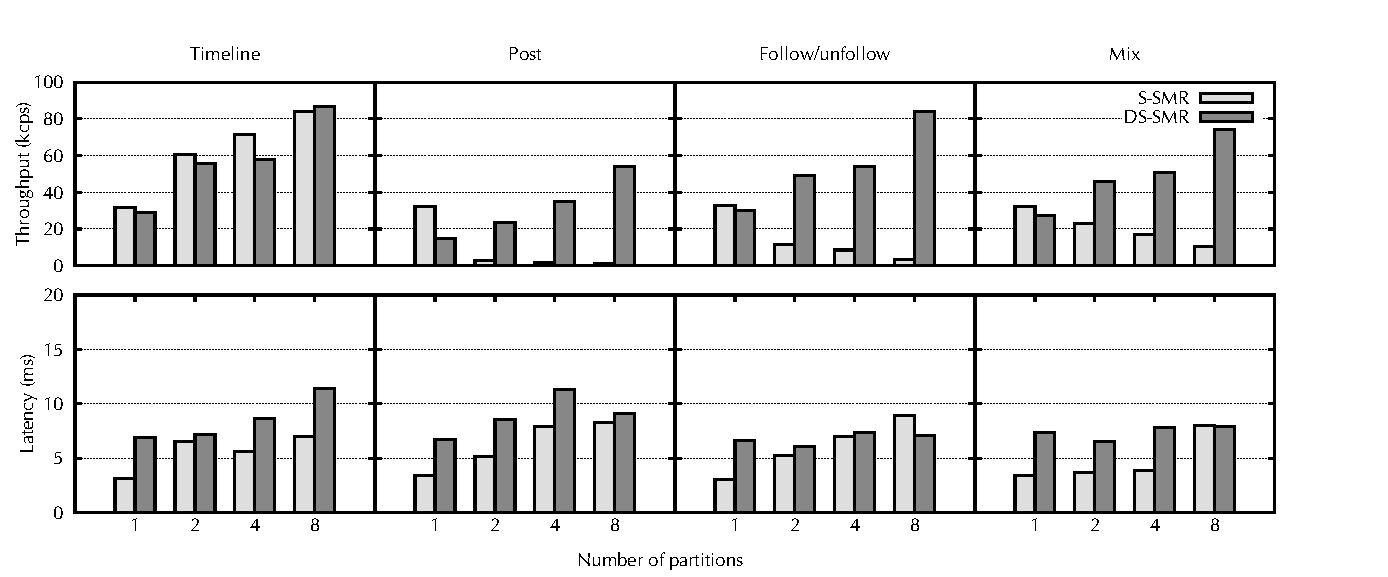
\includegraphics[width=1.08\linewidth]{figures/graphs/strong-locality}
\end{minipage}
\caption{Results of \appname\ running with \ssmr\ and \dssmr{}. Throughput is shown in thousands of commands per second (kcps).}
\label{fig:strongloc}
\end{figure*}

\begin{table*}[htp]
\vspace{10mm}
\caption{Absolute values of \appname\ running \ssmr\ and \dssmr{}.}
\centering
\begin{tabular}{|l|c|c|c|c|c|c|c|c|c|c|c|c|c|c|c|c|} \hline
         & \multicolumn{4}{|c|}{Timeline}  &  \multicolumn{4}{|c|}{Post}   &  \multicolumn{4}{|c|}{Follow/unfollow}  &  \multicolumn{4}{|c|}{Mix}    \\ \hline
         & 1     & 2     & 4     & 8       & 1     & 2     & 4   & 8    & 1     & 2     & 4       & 8           & 1     & 2     & 4     & 8     \\ \hline\hline
         & \multicolumn{16}{|c|}{Throughput (commands per second)} \\ \hline
\ssmr\   & 31757 & 60699 & 71274 & 84065   & 32151 & 2884  & 1894  & 1200  & 32541 & 11476 & 8580    & 3371          & 32151 & 22803 & 16822 & 10657 \\ \hline
\dssmr\  & 28882 & 55925 & 57900 & 86685   & 14874 & 23295 & 35188 & 54250 & 30215 & 48976 & 54025   & 83880         & 27101 & 45686 & 50671 & 74257 \\ \hline\hline
         & \multicolumn{16}{|c|}{\textbf{Throughput rate = \dssmr\ tput / \ssmr\ tput}} \\ \hline
         & \textbf{0.91} & \textbf{0.92}  & \textbf{0.81} & \textbf{1.03}     & \textbf{0.46}   & \textbf{8.08}   & \textbf{18.48}  & \textbf{45.00} & \textbf{0.93} & \textbf{4.27} & \textbf{6.30} & \textbf{24.88} & \textbf{0.84} & \textbf{2.00} & \textbf{3.01} & \textbf{6.97} \\ \hline\hline
         & \multicolumn{16}{|c|}{Latency (milliseconds)} \\ \hline
\ssmr\   & 3.1 & 6.6 & 5.6 & 7.0  & 3.4 & 5.2  & 7.9  & 8.3  & 3.0  & 5.2  & 7.0  & 8.8  & 3.4  & 3.7  & 3.8  & 7.9  \\ \hline
\dssmr\  & 6.9 & 7.1 & 8.6 & 11.4 & 6.7 & 8.6  & 11.3 & 9.1  & 6.6  & 6.1  & 7.4  & 7.0  & 7.3  & 6.5  & 7.8  & 7.9  \\ \hline
\end{tabular}
\label{tbl:results}
\vspace{10mm}
\end{table*}%

\subsection{Environment setup and configuration parameters}
\label{sec:evaluation:setup}

We conducted all experiments on a cluster that had two types of nodes: (a) HP SE1102 nodes, equipped with two Intel Xeon L5420 processors running at 2.5 GHz and with 8 GB of main memory, and (b) Dell SC1435 nodes, equipped with two AMD Opteron 2212 processors running at 2.0 GHz and with 4 GB of main memory. The HP nodes were connected to an HP ProCurve 2920-48G gigabit network switch, and the Dell nodes were connected to another, identical switch. Those switches were interconnected by a 20 Gbps link.
All nodes ran CentOS Linux 7.1 with kernel 3.10 and had the OpenJDK Runtime Environment~8 with the \mbox{64-Bit} Server VM (build 25.45-b02).
%We kept the clocks synchronized using NTP in order to measure latency components involving events in different computers.

For the experiments, we use the following workloads:
Timeline (composed only of getTimeline requests),
Post (only post requests),
Follow/unfollow (50\% of follow requests and 50\% of unfollow), and
Mix (7.5\% post, 3.75\% follow, 3.75\% unfollow, and 85\% getTimeline).

\subsection{Results }
\label{sec:evaluation:strongloc}

% THROUGHPUT

We can see in Figure~\ref{fig:strongloc} and Table~\ref{tbl:results} the results achieved with \appname{}.
%, running with a strong-locality workload.
For the Timeline workload, the throughput with \dssmr\ and \ssmr\ are very similar.
This happens because getTimeline requests are optimized to be single-partition:
all posts in a user's timeline are stored along with the User object.
%Every getTimeline requests accesses a single User object (of the user whose timeline is being requested).
This is the ideal workload for \ssmr{}.
In \dssmr{}, the partitioning does not change, and consulting the oracle becomes unnecessary thanks to the local cache at each client.
This happens because there are no other commands in the Timeline workload.

In the Post workload, every command accesses up to all partitions in the system, which is the worst case for \ssmr{}: the more partitions are involved in the execution of a command, the worst is the system's performance.
We can see that the throughput of \ssmr\ decreases significantly as the number of partitions increases.
For \dssmr{}, we can see that the system throughput scales with the number of partitions.
This happens because User objects that are accessed together, but which are in different partitions, are moved to the same partition based on the interests of the users.
In the case of post command on 2 partitions, the number of move commands started ~3kcps, over 23kps of throughput, then reduced to less than 0.1kcps over time.\fxnote[draft]{Add ratio of move command}
As the execution proceeds, this leads to a lower rate of multi-partition commands, which allows throughput to scale.
As a result the throughput improvement of \dssmr{} with respect to \ssmr\ increases over time.
With eight partitions, \dssmr{} sports a performance that is 45 times that of \ssmr!

With the Follow/unfollow workload, the system performs in a similar way to that observed with the Post workload.
The difference is that each follow or unfollow request accesses only two User objects, whereas every post request may affect an unbounded number of users.
For this reason, each follow/unfollow command is executed at most by two partitions in \ssmr{}.
In \dssmr{}, a single move command is enough to have all User objects affected by such a command in the same partition.
For this reason, both replication techniques have better throughput under the Follow/unfollow workload than with Post.
As with the Post workload, \dssmr{}'s advantage over \ssmr\ increases with the number of partitions, reaching up to almost 25 times with eight partitions.

We approximate a realistic distribution of commands with the Mix workload.
With such a workload, \ssmr\ does not perform as bad as in the Post or Follow/unfollow workloads, but the system throughput still decreases as partitions are added.
As with the other workloads, \dssmr\ scaled under the Mix workload.
With eight partitions, it reached 74~kcps (thousands of commands per second), fairly close to the ideal case (the Timeline workload), where \dssmr\ reached 86~kcps.
Under the Mix workload, \ssmr\ had less than 33~kcps in the best case (one partition) and around 10~kcps with eight partitions.
In the configuration with eight partitions, \dssmr\ reaches almost seven times \ssmr's throughput.

Latency values with \dssmr\ are higher than with \ssmr{}.
This was expected for two reasons. First, there is an extra group of servers (the oracle) to communicate with.
Second, executing a command often means moving all accessed objects to the same partition.
Taking this into account, we consider the (often slight) increase in latency observed with \dssmr\ a low price to pay for the significant increase in throughput and the scalability that \dssmr\ brought to the system; with \ssmr{}, the system did not scale with multi-partition commands.



%\subsection{Results for weak locality}
%\label{sec:evaluation:weakloc}
%!TEX root =  main.tex
\section{Related work}
\label{sec:rw}

State machine replication~\cite{Kapritsos:2012um, kotla2004htbft, Lam78, santos2013htsmr, Sch90} provides strong consistency guarantees, which come from total order and deterministic execution of commands.
%Deterministic execution is usually ensured by having every replica execute commands sequentially.
Since consistent ordering is fundamental for SMR, some authors proposed to optimize the ordering and propagation of commands.
% (i.e., the atomic broadcast layer of the system).
For instance, \cite{kapritsos2010scalable} proposes to divide the ordering of commands between different clusters: each cluster orders only some requests, and then forwards the partial order to every server replica, which then merges the partial orders deterministically into a single total order that is consistent across the system.
In~\cite{biely2012spaxos}, Paxos~\cite{Lamport:1998ea} is used to order commands, but it is implemented in a way that avoids overloading the leader process, which would turn it into a bottleneck.

Multi-threaded execution is a potential source of non-determinism, depending on how threads are scheduled to be executed in the operating system.
Some works attempted to circumvent this problems and come up with a multi-threaded, yet deterministic implementation of SMR.
In \cite{santos2013htsmr}, the authors propose to parallelize the receipt and dispatching of commands, while executing commands sequentially.
In \cite{kotla2004htbft}, application semantics is used to determine which commands can be executed concurrently and still produce a deterministic outcome (e.g., read-only commands).
In \cite{Kapritsos:2012um}, commands are tentatively executed in parallel.
After the parallel execution, replicas verify whether they reached a consistent state; if not, commands are rolled back and re-executed sequentially.

Many database replication schemes aim at achieving high throughput by relaxing consistency, that is, they do not ensure linearizability.
In deferred-update replication \cite{chundi96dur, kobus2013hybrid, sciascia2012sdur, SousaOMP01}, replicas commit read-only transactions immediately, not always synchronizing with each other.
Although this indeed improves performance, it allows non-linearizable executions.
Database systems usually ensure serializability \cite{BHG87} or snapshot isolation \cite{LinKJPA09}, which do not take into account real-time precedence of different commands among different clients. 
For some applications, these consistency levels may be enough, allowing the system to scale better, but services that require linearizability cannot be implemented with such techniques.

Efforts to make linearizable systems scalable have been made in the past~\cite{bezerra2014ssmr, corbett2013spanner, Glendenning2011, hoang2016, Marandi11}.
In \cite{Glendenning2011}, the authors propose a scalable key-value store based on DHTs, ensuring linearizability, but only for requests that access the same key. 
In \cite{Marandi11}, variant of SMR is proposed in which data items are partitioned but commands have to be totally ordered.
Spanner~\cite{corbett2013spanner} uses a separate Paxos group per partition and, to ensure strong consistency across partitions, clocks are assumed to be synchronized.
Although the authors say that Spanner works well with GPS and atomic clocks, if clocks become out of synch beyond tolerated bounds, correctness is not guaranteed.
\ssmr{}~\cite{bezerra2014ssmr} ensures consistency across partitions without any assumption about clock synchronization, but relies on a static partitioning of the state.
\dssmr{}~\cite{hoang2016} extends \ssmr\ by allowing state variables to migrate across partitions in order to reduce multi-partition commands.
However, \dssmr{} implements repartitioning in a very simple way that does not perform very well in scenarios with weak locality.
\dynastar\ improves on \dssmr\ by employing well-known graph partitioning techniques to decide where each variable should be.
Moreover, \dynastar\ dillutes the cost of repartitioning by moving variables on-demand, that is, only when they are accessed by some command.

Graph partitioning is an interesting problem with many proposed solutions~\cite{Abou-Rjeili:2006,kernighan1970efficient,hendrickson2000graph}.
In this work, we do not introduce a new graph partitioning solution, but instead we use a well-known one (METIS~\cite{Abou-Rjeili:2006}) to partition the state of a service implemented with state machine replication.
Similarly to \dynastar{}, Schism~\cite{curino2010sch} and Clay~\cite{SerafiniTEPAS16} also use graph-based partitioning to decide where to place data items in a transactional database.
In either case, not much detail is given about how to handle repartitioning dynamically without violating consistency.
Sword~\cite{quamar2013sword} is another graph-based dynamic repartitioning technique.
It uses a hypergraph partitioning algorithm to distribute rows of tables in a relational database across database shards.
Sword does not ensure linearizability and it is not clear how it implements repartitions without violating consistency.
E-Store~\cite{taft2014est} is yet another repartitioning proposal for transactional databases.
It repartitions data according to access patterns from the workload.
It strives to minimize the number of multi-partition accesses and is able to redistribute data items among partitions during execution.
E-Store assumes that all non-replicated tables form a tree-schema based on foreign key relationships.
This has the drawback of ruling out graph-structured schemas and \mbox{$m$-$n$} relationships.
\dynastar\ is a more general approach that works with any kind of relationship between data items, while also ensuring linearizability.

Some replication schemes are ``dynamic'' in that they allow the membership to be reconfigured during execution (e.g., \cite{birman2010dsr,dustdar2007soc,guessoum2003dar}).
For instance, a multicast layer based on Paxos can be reconfigured by adding or removing acceptors. 
These systems are dynamic in a way that is orthogonal to what \dynastar\ proposes.
%\dynastar\ consists of allowing the \emph{state partitioning}, that is, which state variables belong to which partition, to change dynamically.
%The greatest challenge that is addressed by \dynastar\ is how to provide such a solution, with a dynamic partitioning oracle, while ensuring a very strong level of consistency (linearizability), as variables are created, deleted, and moved across partitions, based on the access patterns of the workload.


\section{Conclusion}
\label{sec:conclusion}

This work introduces S-SMR, a scalable variant of the well-known state-machine replication technique. 
S-SMR differs from previous related works in that it allows throughput to scale with the number of partitions without weakening consistency. 
To evaluate S-SMR, we developed the Eyrie library and implemented Volery, a Zookeeper clone, with Eyrie.
Our experiments demonstrate that in deployments with 8 partitions (the largest configuration we can deploy in our infrastructure) and under certain workloads, throughput experienced an 8-time improvement, resulting in ideal scalability.
Moreover, Volery's throughput proved to be significantly higher than Zookeeper's.

%removed acks because of double-blind!!! re-enable after getting accepted
\section*{Acknowledgements}

This work was supported in part by the Swiss National Science Foundation under grant number 146404.

%\pagebreak

% why did you have this vvv ?
%\bibliographystyle{splncs03}
\bibliographystyle{ieeetr}
\bibliography{references}
\newpage


\end{document}